\documentclass[a4paper]{article}
\usepackage[margin=0.8in]{geometry}
\usepackage[operators]{cryptocode}
\usepackage{tikz}
\usepackage{wrapfig}
\renewcommand\O[1]{\ensuremath{\mathsf{#1}}}
\newcommand{\M}[1]{\ensuremath{\text{\texttt{#1}}}}
\newcommand{\n}[1]{\ensuremath{\mathit{#1}}}
\tikzstyle{package} = [inner sep=1pt,align=center,rounded corners,draw,minimum width=2cm,minimum height=1cm,font=\small]
\tikzstyle{onarrow} = [inner sep=1pt,font=\scriptsize,anchor=east,at end,xshift=-0.1mm,align=left,fill=white]
%\title{Proof: Modularize}
\begin{document}
%\maketitle
\vspace{-5cm}

\section{Example of a code equivalence proof}
%\subsection{monprfreal Game}

\begin{wrapfigure}{R}{0.6\textwidth}
\vspace{-0.7cm}
\begin{pcvstack}
\underline{\underline{monprfreal Game}}\\
\scalebox{0.8}{
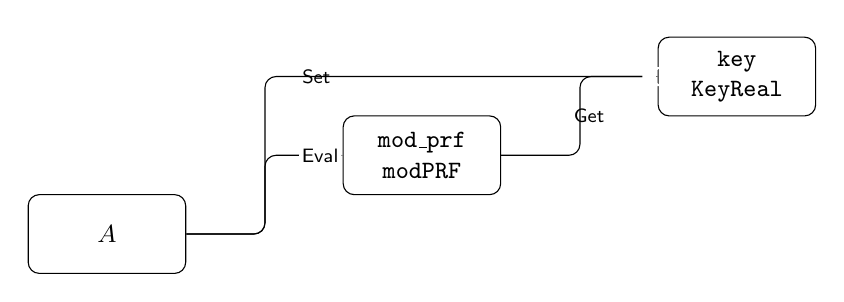
\begin{tikzpicture}
\node[align=center,package,fill=white] (node1) at (0, 0) {\M{key}\\\M{KeyReal}};
\node[align=center,package,fill=white] (node0) at (-4, -1) {\M{mod\_prf}\\\M{modPRF}};
\draw[-latex,rounded corners] (node0) -- ($(node0.east) + (1,0)$) |- node[onarrow] {\hspace{-8.6cm}\O{Set}} (node1);
\node[package] (nodea) at (-8, -2) {$A$};
\draw[-latex,rounded corners] (nodea) -- ($(nodea.east) + (1,0)$) |- node[onarrow] {\O{Eval}} (node0);
\draw[-latex,rounded corners] (nodea) -- ($(nodea.east) + (1,0)$) |- node[onarrow] {\begin{minipage}{0.01cm}\vspace{1cm}
\hspace{-1cm}
																																												\O{Get}
																																										\end{minipage}
																																												} (node1);
\end{tikzpicture}
}
\pcvspace
\begin{pchstack}
\begin{pcvstack}\underline{\underline{\M{mod\_prf}}}\\\begin{pchstack}
\procedure{\O{Eval}(h)}{
\pcif \n{ltk} = \O{none}(\O{Bits("n")}) \pcthen\\
\pcind\n{ltk\_} \stackrel{1}{\sample} \O{Bits("n")}\\
\pcind \n{ltk} \gets \O{some}(\n{ltk\_})\\
 \n{ltk\_} \gets \O{unwrap}(\n{ltk})\\
 \n{k} \gets \O{prf}(\n{ltk\_}, \n{h})\\
\n{\_} \stackrel{\mathsf{\tiny{invoke}}}{\gets} \O{Set}(\n{k}, \n{h}) \pccomment{Pkg: key}
}
\pchspace
\end{pchstack}\end{pcvstack}

\begin{pcvstack}\underline{\underline{\M{key}}}\\
%\begin{pchstack}
\procedure{\O{Set}(k, h)}{
\pcif \n{K}[\n{h}] = \O{none}(\O{Bits("n")}) \pcthen\\
\pcind \n{K}[\n{h}] \gets \O{some}(\n{k})
}
\pcvspace
\procedure{\O{Get}(h)}{
 \pcreturn \O{unwrap}(\n{K}[\n{h}])\\
}
%\pchspace
%\end{pchstack}
\end{pcvstack}

\end{pchstack}
\end{pcvstack}
\vspace{-0.5cm}
\end{wrapfigure}


When writing SSP-style proofs, we often write PRF assumptions modularly. For example, we ``move out'' the outputs of the PRF into a key package (see figure on the right). Security of a PRF can then be defined by using an real key package (see figure on the right) or an ideal key package (not depicted---instead of writing $k$ to $K[h]$, it samples a random value instead) and requiring indistinguishability between the two modular games described by using a real and an ideal key package, respectively.


In this note, we want to consider the case that we want to show via reduction that this SSP-style modular PRF notion is implied by a standard monolithic PRF security notion. In this case, we write a reduction (reductionPRF on the right) 

\begin{wrapfigure}{R}{0.5\textwidth}
\vspace{-0.7cm}
\begin{pcvstack}
\underline{\underline{monprfreal Game}}\\
\scalebox{0.8}{
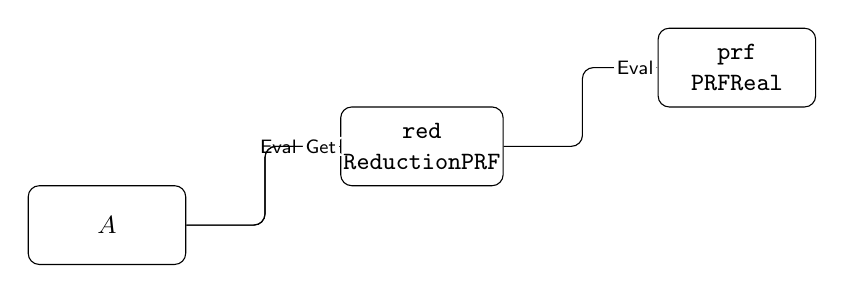
\begin{tikzpicture}
\node[align=center,package,fill=white] (node0) at (0, 0) {\M{prf}\\\M{PRFReal}};
\node[align=center,package,fill=white] (node1) at (-4, -1) {\M{red}\\\M{ReductionPRF}};
\draw[-latex,rounded corners] (node1) -- ($(node1.east) + (1,0)$) |- node[onarrow] {\O{Eval}} (node0);
\node[package] (nodea) at (-8, -2) {$A$};
\draw[-latex,rounded corners] (nodea) -- ($(nodea.east) + (1,0)$) |- node[onarrow] {\hspace{-1.5cm}\O{Eval}} (node1);
\draw[-latex,rounded corners] (nodea) -- ($(nodea.east) + (1,0)$) |- node[onarrow] {\O{Get}} (node1);
\end{tikzpicture}
}
\pcvspace
\begin{pchstack}
\begin{pcvstack}\underline{\underline{\M{red}}}\\
\procedure{\O{Eval}(h)}{
\n{y} \stackrel{\mathsf{\tiny{invoke}}}{\gets} \O{Eval}(\n{h}) \pccomment{Pkg: prf} \\
\n{K}[\n{h}] \gets \O{some}(\n{y})
}
\pcvspace
\procedure{\O{Get}(h)}{
 \pcreturn \O{unwrap}(\n{K}[\n{h}])\\
}

\end{pcvstack}

\begin{pcvstack}\underline{\underline{\M{prf}}}\\\begin{pchstack}
\procedure{\O{Eval}(h)}{
\pcif \n{ltk} = \O{none}(\O{Bits("n")}) \pcthen\\
\pcind\n{ltk\_} \stackrel{1}{\sample} \O{Bits("n")}\\
\pcind \n{ltk} \gets \O{some}(\n{ltk\_})\\
 \pcreturn \O{prf}(\O{unwrap}(\n{ltk}), \n{h})\\
}
\pchspace
\end{pchstack}\end{pcvstack}

\end{pchstack}
\scalebox{0.7}{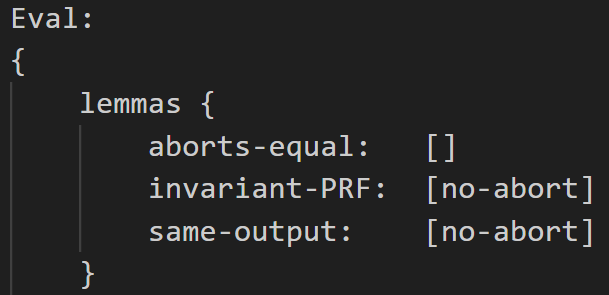
\includegraphics{lemmas.png}}
\pcvspace
\scalebox{0.7}{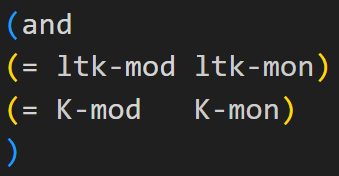
\includegraphics{invariant-code.png}}
\pchspace
\scalebox{0.7}{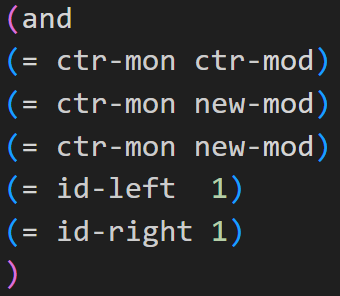
\includegraphics{randomness-mapping.png}}
\end{pcvstack}
\vspace{-1.2cm}
\end{wrapfigure}

\noindent
and need to show that the reduction composed with the real monolithic PRF game (monprfreal on the right) behaves in the same way as the real modular PRF game (modprfreal on the right). Moreover, we need to prove the analogous statement for the ideal PRF games. In this note, we focus on the real case only and omit the ideal case.



%\subsection{monprfideal Game}
%\input{CompositionGraph_monprfideal.tex}
%\end{center}
%\begin{center}
%\begin{pchstack}
%\begin{pcvstack}\underline{\underline{\M{red}}}\\
\procedure{\O{Eval}(h)}{
\n{y} \stackrel{\mathsf{\tiny{invoke}}}{\gets} \O{Eval}(\n{h}) \pccomment{Pkg: prf} \\
\pcif \n{K}[\n{h}] = \O{none}(\O{Bits("n")}) \pcthen\\
\pcind \n{K}[\n{h}] \gets \O{some}(\n{y})\\
}
\pcvspace
\procedure{\O{Get}(h)}{
 \pcreturn \O{unwrap}(\n{K}[\n{h}])\\
}

\end{pcvstack}

%\pchspace
%\begin{pcvstack}\underline{\underline{\M{prf}}}\\\begin{pchstack}
\procedure{\O{Eval}(h)}{
\pcif \n{ltk} = \O{none}(\O{Bits("n")}) \pcthen\\
\pcind\n{ltk\_} \stackrel{1}{\sample} \O{Bits("n")}\\
\pcind \n{ltk} \gets \O{some}(\n{ltk\_})\\
 \pcreturn \O{prf}(\O{unwrap}(\n{ltk}), \n{h})\\
}
\pchspace
\end{pchstack}\end{pcvstack}

%\end{pchstack}
%\end{center}
%\subsection{modprfideal Game}
%\begin{center}
%\input{CompositionGraph_modprfideal.tex}
%\end{center}
%\begin{center}
%\begin{pchstack}
%\begin{pcvstack}\underline{\underline{\M{mod\_prf}}}\\\begin{pchstack}
\procedure{\O{Eval}(h)}{
\pcif \n{ltk} = \O{none}(\O{Bits("n")}) \pcthen\\
\pcind\n{ltk\_} \stackrel{1}{\sample} \O{Bits("n")}\\
\pcind \n{ltk} \gets \O{some}(\n{ltk\_})\\
 \n{ltk\_} \gets \O{unwrap}(\n{ltk})\\
 \n{k} \gets \O{prf}(\n{ltk\_}, \n{h})\\
\n{\_} \stackrel{\mathsf{\tiny{invoke}}}{\gets} \O{Set}(\n{k}, \n{h}) \pccomment{Pkg: key}
}
\pchspace
\end{pchstack}\end{pcvstack}

%\pchspace
%\begin{pcvstack}\underline{\underline{\M{key}}}\\
%\begin{pchstack}
\procedure{\O{Set}(k, h)}{
\pcif \n{K}[\n{h}] = \O{none}(\O{Bits("n")}) \pcthen\\
\pcind \n{K}[\n{h}] \gets \O{some}(\n{k})
}
\pcvspace
\procedure{\O{Get}(h)}{
 \pcreturn \O{unwrap}(\n{K}[\n{h}])\\
}
%\pchspace
%\end{pchstack}
\end{pcvstack}

%\end{pchstack}
%\end{center}

The main idea is a proof by induction over the number of oracle class. We define an invariant on the states of the two games which holds in the beginning of the game and such that for all oracles Set, Eval and Get, the following holds:
\begin{itemize}
\item If the invariant holds before an oracle call, then one game aborts iff the other game aborts.
\item If the invariant holds before an oracle call and none of the two game aborts, then the invariant holds after an oracle call as well.
\item If the invariant holds before an oracle call and none of the two game aborts, then the oracle calls in both games return the same answer to the adversary.
\end{itemize}
We depict these three lemmas for the Eval oracle on the right. The SMT solver proves these lemmas automatically, but needs the invariant to be defined by the user. In this case, the invariant that we define is very simple, namely, the two games need to have the same content in table $K$ (K-mod and K-mon) and variable $\mathsf{ltk}$ (ltk-mod and ltk-mon). SMTlib uses a style where the operator comes first and the arguments next, so (= K-mod K-mon) refers to K-mod being equal to K-mon. Additionally, the state invariant requires the counters for randomness to be equal which brings us to the topic of randomness. Since the games perform some sampling (sampling of $\mathsf{ltk}$), we need a randomness relation to say that they use the \emph{same} randomness (as else, they would compute different PRF values based on different $\mathsf{ltk}$). Here, we say that both randomness samplings with identifier 1 are equal. (= ctr-mod ctr-mon) refers to equality of the counters in the state (which our invariant sais are equal) and icr-mod and icr-mon refer to the incremented counters in this oracle calls which are equal to ctr-mon and ctr-mod, since there was no randomness sampling before within this oracle call. (TODO: explain more)


%\section{Equivalence between modprfreal and monprfreal}
\end{document}






